\setchapterpreamble[u]{\margintoc}
\chapter{Perturbation theory}

This subject proposed solutions for problemsthat can not be solved exactly.

\section{Introduction}

We are going to recall our hamiltonian for the schrodinguer wave equation.

\begin{equation}
  H \psi(x,y,z,t) =i \hbar \frac{\partial \psi(x,y,z,t)}{\partial t}
\end{equation}

Where H is non depending on time. Let's assume once more that the solution of this equation looks like:

\begin{equation}
  \psi(x,y,z,t) = \phi(x,y,z) e^{-i\frac{E}{\hbar}t}
\end{equation}

Then:

\begin{equation}
  \begin{array}{c}
  e^{-i\frac{E}{\hbar}t}(H \phi(x,y,z)) = E e^{-i\frac{E}{\hbar}t} \phi(x,y,z)
  \\

  \\
  H \phi(x,y,z) = E \phi(x,y,z)
  \end{array}
\end{equation}

As we have been doing since the beginning of the semester. But then how can a state go to the ground state if the states are stationary in time?. We need to include in our equation the variation with time.

The change of states must be solutions to:

\begin{equation}
  V(\tau) = V(r) + \delta V(r,t)
\end{equation}

This second term is 0 for small changes, But

\begin{equation}
  \bra{n=2,j=1,m=1}\delta V(r,t)\ket{n=1,j=0,m=0} \neq 0
\end{equation}

For as the perturbation is going to be a function of r only. An example of this is a circuit with a gas chamber, as the one show in METER FIJURA. When the switch is open the gas is stable, onece we closed the switch the gas gets excited andif we closed the switch the gas dexcites. For as this switch control is going to be defined by a function $\delta V(r)$.

% METER FIGURA

\section{Equation with perturbation}

We are going to assume that $H_0$ can be solved exactly. It can be any know hamiltonian, not necessarily the solutions for the hydrogen atom. We say that $H_0$ can be solved in:

\begin{equation}
  \begin{array}{c}
    n=0,1,2,3,\dots
    \\

    \\
    E_0 \leq E_1 \leq E_2 \dots
    \\

    \\
    H_0 \ket{n} = E_n \ket{n}
  \end{array}
\end{equation}

We are going to assume that the perturbation is small, so we can write the hamiltonian as:

\begin{equation}
  H = H_0 + \lambda V_1(r)
\end{equation}

Where $\lambda$ is a small number. This can not be exactly solved. Our equation is going to look like:

\begin{equation}
  (H_0+\lambda_1 V_1) \phi = E_\phi\phi
\end{equation}

Where I'am going to define the eigen-values as:

\begin{equation}
  E_\phi =\sum_{k=0}^{\infty} \lambda^k \mu_k
\end{equation}

I'm also going to redefine the eigen-vectors as:

\begin{equation}
  \ket{\phi} = \sum_{k=0}^{\infty} \lambda^k \ket{\phi_k}
\end{equation}

We need to solve for every k.

For some range of $\lambda$ the next assumption must be true.

\begin{equation}
  (H_0 + \lambda_1V_1) (\ket{\phi_0}+\lambda\ket{\phi_1}+...) = (\mu_0 + \lambda\mu_1 + \lambda^2\mu_2 + \dots)(\ket{\phi_0}+\lambda\ket{\phi_1}+...)
\end{equation}

This equation must be true term by term in $\lambda$.

\begin{equation}
  \begin{array}{lc}
    \lambda^0 => & H_0 \ket{\phi_0} = \mu_0 \ket{\phi_0}
    \\

    \\
    \lambda^1 => & H_0 \ket{\phi_1} + V_1 \ket{\phi_0} = \mu_0\ket{\phi_1} + \mu_1\ket{\phi_0}
    \\

    \\
                 & (H_0-\mu_0) \ket{phi_1} = (\mu_0 - V_1) \ket{\phi_0}
    \\

    \\
    \lambda^2 => & H_0 \ket{\phi_2} + V_1 \ket{\phi_1} = \mu_0\ket{\phi_2} + \mu_1\ket{\phi_1} + \mu_2\ket{\phi_0}
    \\

    \\
                 & (H_0-\mu_0) \ket{\phi_2} = (\mu_1 - V_1) \ket{\phi_1} + \mu_2\ket{\phi_0}
  \end{array}
\end{equation}

If we solved for the first term:

\begin{equation}
  \begin{array}{c}
    H_0 \ket{\phi_0}= \mu_0 \ket{\phi_0}
    \\

    \\
    E_n \ket{\phi_0} = \mu_0 \ket{\phi_0}
    \\

    \\
    \ket{\phi_0} = \ket{n}
    \\

    \\
    \mu_0 = E_n
  \end{array}
\end{equation}

We can use this result to solve the next term.

\begin{equation}
\begin{array}{c}
  (H_0 - \mu_0)\ket{\phi_1} = (\mu_1 - V_1)\ket{\phi_0}
  \\

  \\
  (H_0 - E_n)\ket{\phi_1} = (\mu_1 - V_1)\ket{n}
\end{array}
\end{equation}

We are going to solve it multiplying by $\bra{n}$ at both sides of the equation.

\begin{equation}
  \begin{array}{c}
    \bra{n}(H_0 - E_n)\ket{\phi_1} = \bra{n}\mu_1\ket{n} - \bra{n}V_1\ket{n}
    \\

    \\
    E_n\bra{n}\ket{\phi_1} - E_n\bra{n}\ket{\phi_1} = \mu_1 - \bra{n}V_1\ket{n}
    \\

    \\
    \mu_1 = \bra{n}V_1\ket{n}
  \end{array}
\end{equation}

We can rewrite $\ket{\phi_1}$ as a linear combination of the eigen-vectors of $H_0$.

\begin{equation}
  \label{13.16}
  \ket{\phi_1} = \sum_{m=0}^{\infty} C_{1,m} \ket{m}
\end{equation}

If we plug this in the equation above:

\begin{equation}
\begin{array}{c}
  (H_0 - E_n) (\sum_{m} C_{1,m} \ket{m}) = \mu_1 \ket{n} - V_1 \ket{n}
  \\

  \\
  \sum_{m} C_{1,m} (H_0 - E_n) \ket{m} = \mu_1 \ket{n} - V_1 \ket{n}
  \\

  \\
  \sum_{m} C_{1,m} (E_m - E_n) \ket{m} = \mu_1 \ket{n} - V_1 \ket{n}
\end{array}
\end{equation}

We are going to solve taking the inner product with k.

\begin{equation}
  \begin{array}{c}
    \sum_{m} C_{1,m} (E_m-E_n) \braket{k}{m} = \mu_1 \braket{k}{n} - V_1 \braket{k}{n}
    \\

    \\
    C_{1,k} (E_k - E_n) = \mu_1 \delta_{k,n} - \bra{k}V_1\ket{n}
    \\

    \\
    C_{1,k} = \frac{-\bra{k}V_1\ket{n}}{E_k-E_n} ; k \neq n
  \end{array}
\end{equation}

Our eigen-vector looks like:

\begin{equation}
  \ket{\phi_1} = C_{1,n}\ket{n} + \sum_{m \neq n} \frac{-\bra{m}V_1\ket{n}}{E_m - E_n} \ket{m}
\end{equation}

All the eigen-values and eigen-vectors look like:

\begin{equation}
  \begin{array}{c}
  E_{\phi} = E_n + \lambda\bra{n}V_1\ket{n} + ...
  \\

  \\
  \ket{\phi} = (1+\lambda C_1) \ket{n} + \lambda \sum_{m \neq n} \frac{\bra{m}V_1\ket{n}}{E_n - E_m}\ket{m} + ...
  \end{array}
\end{equation}

Where $C_1$ can be found using normalization. Sometimes the first orderaproximation is zero, then we have to use the second order aproximation.

\begin{equation}
  \begin{array}{c}
    (H_0 - E_n) \ket{\phi_2} = \mu_1 \ket{\phi_1} - V_1 \ket{\phi_1} + \mu_2 \ket{n}
  \end{array}
\end{equation}

Let's assume again solutions like the ones from \ref{13.16} for $\ket{\phi_2}$.

\begin{equation}
\begin{array}{c}
  \sum_{k} C_{2,k}(H_0-E_n)\ket{k} = \sum_{l} C_{1,l} (\mu_1 - V_1)\ket{l} + \mu_2 \ket{n}
  \\

  \\
  \bra{m} \left[\sum_{k} C_{2,k}(H_0-E_n)\ket{k} = \sum_{l} C_{1,l} (\mu_1 - V_1)\ket{l} + \mu_2 \ket{n}\right]
  \\

  \\
  \sum_k C_{2,k}(E_k -E_n)\delta_{k,m} = \sum_l C_{1,l} (\mu_1 \delta_{m,l} - \bra{m}V_1\ket{l}) + \mu_2 \delta_m,n
\end{array}
\end{equation}

If m = n:

\begin{equation}
\begin{array}{c}
  0 = \mu_1 C_{1,n} - \sum_l C_{1,l} \bra{n}V_1\ket{l} + \mu_2
  \\

  \\
  0 = \mu_1 C_{1,n} - C_{1,n}\bra{n}V_1\ket{n} - \sum_{l\neq n} C_{1,l} \bra{n}V_1\ket{l} + \mu_2
  \\

  \\
  \mu_2 = \sum_{l\neq n} C_{1,l} \bra{n}V_1\ket{l} = \sum_{l\neq n} \frac{\bra{l}V_1\ket{n} \bra{n}V_1\ket{l}}{E_n - E_l}
\end{array}
\end{equation}

If $m \neq n$:

\begin{equation}
  \begin{array}{c}
    C_{2,k}= \frac{\mu_1 C_1,k - \sum_l \bra{m}V_1\ket{l}}{E_m - E_n}
  \end{array}
\end{equation}

And you can keep going with this process.

\section{Degenerate States}

If we have more than one state with the same energ, we can have something like:

\begin{equation}
  \begin{array}{c}
    \ket{\phi_0} = C_n \ket{n} +C_{n+1}\ket{n+1}
    \\

    \\
    \mu_0 = E_n = E_{n+1}
  \end{array}
\end{equation}

Equation \ref{13.14} is going to look like:

\begin{array}{c}
  (H_0-E_n) = (\mu_1-V_1)\left[C_n \ket{n} + C_{n+1}\ket{n+1}\right]
\end{array}

We can still solve this multiplying by $\bra{n}$ and $\bra{n+1}$, which is going to give as two equations that are similar to \ref{13.15}.

\begin{equation}
\begin{array}{c}
  0 = \mu_1 C_n - C_n \bra{n}V_1\ket{n} - C_{n+1} \bra{n}V_1\ket{n+1}
  \\

  \\
  0 = \mu_1 C_{n+1} - C_{n+1} \bra{n+1}V_1\ket{n+1} - C_n \bra{n+1}V_1\ket{n}
\end{array}
\end{equation}

If we look at this system of equation in a matrix system we get:

\begin{equation}
  \begin{array}{c}
    \begin{bmatrix}
      \bra{n}V_1\ket{n} & \bra{n}V_1\ket{n+1}\\
      \bra{n+1}V_1\ket{n} & \bra{n+1}V_1\ket{n+1}
    \end{bmatrix}
    \begin{bmatrix}
      C_n\\
      C_{n+1}
    \end{bmatrix}
    = \mu_1
    \begin{bmatrix}
      C_n\\
      C_{n+1}
    \end{bmatrix}
  \end{array}
\end{equation}

This implies that $\mu_1$ is an eigenvalue of the matrix where the eigenvectors are the coefficients.

\section{Proton as a sphere}

We've been assuming that the proton is a point particle all this time, but we know it is not. We are going to assume that the proton is a sphere with a charge distribution $\rho$.

\begin{marginfigure}[-4cm]
  \label{figure_proton}
  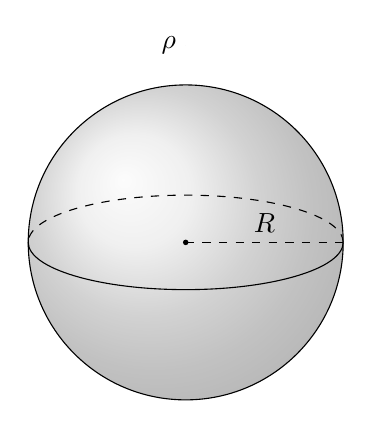
\begin{tikzpicture}
    \shade[ball color = gray!40, opacity = 0.4] (0,0) circle (2cm);
    \draw (0,0) circle (2cm);
    \draw (-2,0) arc (180:360:2 and 0.6);
    \draw[dashed] (2,0) arc (0:180:2 and 0.6);
    \fill[fill=black] (0,0) circle (1pt);
    \draw[dashed] (0,0 ) -- node[above]{$R$} (2,0);
    \filldraw[black] (0,2.5) circle (0pt) node [anchor=east]{$\rho$};
  \end{tikzpicture}
  \caption{Proton as a sphere of radious R and charge density $\rho$}
\end{marginfigure}

The potential of an electron inside the radious of the proton, R, the potential can be calculated aplying Gauss to calculate the electric field.

\begin{equation}
\begin{array}{c}
  \int \vec{E} \cdot d\vec{s} = \frac{Q_{in}}{\epsilon_0}
  \\

  \\
  E 4\pi r^2 = \frac{\rho \frac{4\pi}{3}r^3}{\epsilon_0}
  \\

  \\
  E_{in}  = \frac{e}{4\pi\epsilon_0 R^3} r
\end{array}
\end{equation}

We are going to need also the electric field outside the sphere.

\begin{equation}
\begin{array}{c}
  \int \vec{E} \cdot d\vec{s} = \frac{Q_{in}}{\epsilon_0}
  \\

  \\
  E_{out} = \frac{e}{4\pi \epsilon_0 r^2}
\end{array}
\end{equation}

Now we can define our potential through all space assuming that the potential at the infinite is 0 and knowing that it has to be conitnuous.

\begin{equation}
  \begin{array}{c}
    V(r) - V(\infty) = \int_{r}^{\infty} E_{out} dr
    \\

    \\
    V(r) = \frac{e}{4\pi \epsilon_0} \frac{1}{r}
  \end{array}
\end{equation}

This is the potential that we used for the Hydrogen atom, now we can calculate the potential inside using the continuity of V(r).

\begin{equation}
  \begin{array}{c}
    V(r) - V(R) = \int_{r}^{R} E_{in} dr
    \\

    \\
    V(r) - \frac{e}{4\pi\epsilon_0 R} = \int_{r}^{R} E_{in} dr
    \\

    \\
    V(r) - \frac{e}{4\pi\epsilon_0 R} = \frac{e}{8\pi\epsilon_0 R^3} (R^2-r^2)
    \\

    \\
    V(r) = \frac{e}{8\pi\epsilon_0 R^3} (3R^2-r^2)
  \end{array}
\end{equation}

Knowing the potentials we can find the potential energy that is going to be this potential times the charge of the electron.

\begin{equation}
  U(r) = - e V(r)
\end{equation}

We want to find some potential energy of the form:

\begin{equation}
  U(r) = \left\{\begin{array}{cc}
    V(r) & r \geq R
    \\

    \\
    V(r) + V_1 & r < R
  \end{array}
\end{equation}

Where $V(r)$ is the one from \ref{10.1} and $V_1$ is the perturbation. Then $V_1$ is going to be:

\begin{equation}
  \begin{array}{c}
    V_1 = \frac{e^2}{8\pi\epsilon_0 R^3} (-3R^2+r^2) + \frac{e^2}{4\pi \epsilon_0 r}
    \\

    \\
    V_1 = \frac{e^2}{8\pi\epsilon_0 R^3} \left( -3R^2 + r^2 + \frac{2R^3}{r} \right)
  \end{array}
\end{equation}

Now that we know $V_1$, we can apply the theory in the previous section to calculate the energy. For $E_1$ we can calculate $E_{\phi}$ knowing that $\ket{n}$ = $\ket{n=1,j=0,m=0}$.

\begin{equation}
  \begin{array}{c}
    E_{\phi} = E_1 + \bra{n}V_1\ket{n}
    \\

    \\
    = E_1 + \bra{n=1,j=0,m=0}V_1\ket{n=1,j=0,m=0}
    \\

    \\
    = E_1 + \int_{0}^{2\pi} \int_{0}^{\pi} \int_{0}^{\infty} \psi_{1,0,0}^* V_1 \psi_{1,0,0} r^2 sin\theta dr d\theta d\phi
    \\

    \\
    = E_1 + \int_{0}^{2\pi} d\phi \int_{0}^{\pi} sin\theta d\theta \int_{0}^{\infty} \frac{1}{8\pi b^3} e^{-r/b} \frac{e^2}{8\pi\epsilon_0 R^3}\left(-3R^2+r^2+\frac{2R^3}{r}\right) r^2 dr =
    \\

    \\
    = E_1 + \frac{e^2}{16\pi b^3 \epsilon_0 R^3}  \int_{0}^{\infty} \left[-3R^2e^{-r/b}r^2 + e^{-r/b} r^4 + 2R^3e^{-r/b} r\right] dr
  \end{array}
\end{equation}

Where each integral is:

\begin{equation}
  \begin{array}{c}
    \int_{0}^{R} -3R^2 e^{-r/b}r^2 dr = -3R^2 \int_{0}^{R} e^{-r/b} r^2 dr =
    \\

    \\
    3R^2 (bR^2 e^{-R/b} + 2b^2 R e^{-R/b} + 2b^3 e^{-R/b} - 2b^3)
    \\

    \\
    \int_{0}^{R} e^{-r/b} r^4 dr =
    \\

    \\
    = -b R^4 e^{-R/b} - 4b^2 R^3 e^{-R/b} - 12b^3 R^2 e^{-R/b} - 24b^4 R e^{-R/b} - 24b^5 e^{-R/b} + 24b^5
    \\

    \\
    \int_{0}^{R} 2R^3 e^{-r/b} r dr =
    \\

    \\
    = 2R^3 (-R b e^{-R/b} - b^2 e^{-R/b} + b^2)
  \end{array}
\end{equation}

If we put everything together:

\begin{equation}
  \begin{array}{c}
    E_{\phi} = E_1 +
    \\

    \\
    + \frac{e^2}{8\pi b^3 \epsilon_0 R^3} \left(12b^5+R^3b^2-3R^2b^3-12b^5e^{-R/b}-12b^4Re^{-R/b}-3b^3R^2e^{-R/b}\right) =
    \\

    \\
    E_1 + \frac{e^2 b^2}{8 \pi\epsilon_0 R^3} \left(12 + \frac{R^3}{b^3} - 3\frac{R^2}{b^2} - 12 e^{-R/b} - 12 \frac{R}{b} e^{-R/b} - 3\frac{R^2}{b^2} e^{-R/b}\right)
  \end{array}
\end{equation}

Using \ref{10.5} we get that:

\begin{equation}
  \begin{array}{c}
  E_{\phi} = E_1 + \frac{\pi \epsilon_0 \hbar^4}{2 e^2 m_e R^3} \left(12 + \frac{R^3}{b^3} - 3\frac{R^2}{b^2} - 12 e^{-R/b} - 12 \frac{R}{b} e^{-R/b} - 3\frac{R^2}{b^2} e^{-R/b}\right)
  \end{array}
\end{equation}

We can see that for $R/b \to 0$ the solution is $E_1$ again.

For the second level of energy we are going to assume a mix degeneratestate. We are goint to solve the system getting a 4x4 matrix following the steps from the previous section in degenerate states. The initial state and the energy are going to be defined as:

\begin{equation}
  \begin{array}{c}
    \phi_0 = C_0 \ket{n=2,j=0,m=0} +
    \\
    +C_1 \ket{n=2,j=1,m=1} +
    \\
    +C_2 \ket{n=2,j=1,m=0} +
    \\
    +C_3 \ket{n=2,j=1,m=-1}
    \\

    \\
    \phi_0 = C_0 \ket{1} + C_1 \ket{2} + C_2 \ket{3} + C_3 \ket{4}
    \\

    \\
    \mu_0 = E_2
  \end{array}
\end{equation}

Im going to use this labels just for sake of simplicity. The matrix is going to look like:

\begin{equation}
  \begin{bmatrix}
    \bra{1}V_1\ket{1} & \bra{1}V_1\ket{2} & \bra{1}V_1\ket{3} & \bra{1}V_1\ket{4}\\
    \bra{2}V_1\ket{1} & \bra{2}V_1\ket{2} & \bra{2}V_1\ket{3} & \bra{2}V_1\ket{4}\\
    \bra{3}V_1\ket{1} & \bra{3}V_1\ket{2} & \bra{3}V_1\ket{3} & \bra{3}V_1\ket{4}\\
    \bra{4}V_1\ket{1} & \bra{4}V_1\ket{2} & \bra{4}V_1\ket{3} & \bra{4}V_1\ket{4}
  \end{bmatrix}
\end{equation}

We have to get the eigenvalues of this matrix to get $\mu_1$, but this is matrix is going to be a diagonal matrix because $V_1$ only dependes on r, which implies that the inner product is going to be proportional to $\delta_{j1,j2}\delta_{m1,m2}$ and because all the degenerate states have different j or m values the inner product of every different function with $V_1$ is going to be 0.

\begin{equation}
  \begin{bmatrix}
    \bra{1}V_1\ket{1} & 0 & 0 & 0\\
    0 & \bra{2}V_1\ket{2} & 0 & 0\\
    0 & 0 & \bra{3}V_1\ket{3} & 0\\
    0 & 0 & 0 & \bra{4}V_1\ket{4}
  \end{bmatrix}
\end{equation}

The eigenvalues of this matrix is going to be the own values. Only the exact calculation of one of them is gonna be provided, the rest are solve in a similar way.

\begin{equation}
  \begin{array}{c}
    \bra{1}V_1\ket{1} =
    \\

    \\
    \int_{0}^{2\pi} \int_{0}^{\pi} \int_{0}^{R} \psi_{2,0,0}^* V_1 \psi_{2,0,0} r^2 sin\theta dr d\theta d\phi =
    \\

    \\
    = \frac{e^2}{128b^3\epsilon_0 R^3}\left(-\left(2688b^5+1344Rb^4+288R^2b^3+36R^3b^2+3R^4b\right)\mathrm{e}^{-\frac{R}{2b}}+
    \\
    \left. + 2688b^5-48R^2b^3+4R^3b^2 \right\) =
    \\

    \\
    = \frac{e^2 b^2}{128\epsilon_0 R^3}\left(-(2688+1344\frac{R}{b}+288\frac{R^2}{b^2}+36\frac{R^3}{b^3}+3\frac{R^4}{b^4})e^{-R/2b}+2688-48\frac{R^2}{b^2}+4\frac{R^3}{b^3}\right)
  \end{array}
\end{equation}





Again we can see that if we find the limit $R/b \to 0$ we get that this inner product is 0, recovering the energy without the perturbation. The other energies can be calculated in a similar way.

\begin{equation}
  \begin{array}{c}
    \bra{2}V_1\ket{2} = \bra{3}V_1\ket{3} = \bra{4}V_1\ket{4} =
    \\

    \\
    = \frac{e^2 b^2}{2^{11} 3 \epsilon_0 R^3}\left(-\left(92160 + 46080 \frac{R}{b} + 9216\frac{R^2}{b^2}+960\frac{R^3}{b^3}+48\frac{R^4}{b^4} \right)e^{-R/2b} +
    \\
    \left. + 92160 - 2304 \frac{R^2}{b^2} + 192 \frac{R^3}{b^3} \right)
  \end{array}
\end{equation}

This implies that we have a different energy dephase, one for the state $\ket{1}$ and another for the other states, so both energies are going to change but the ones with j=1 are going to keep being the same value and the one with j=0 is going to separate from the other two. This was expected because $V_1$ only depends on r.

\section{Constant electric field}

Like in the previous section we are going to find the potential first. Let's assume that we have a constant electric potential going into the z direction like the one in Figure \ref{figure_const_elec}.

\begin{marginfigure}[3cm]
  \label{figure_const_elec}
  \begin{tikzpicture}
    \draw[-] (0,0) -- (-1.63,-1.14); % x axis
    \draw[-] (-2,0) -- (2,0); % y axis
    \draw[-] (0,-2) -- (0,2); % z axis
    \filldraw[black] (-1.6,-1.1) circle (0pt) node [anchor=north]{$x$};
    \filldraw[black] (2,0) circle (0pt) node [anchor=north]{$y$};
    \filldraw[black] (0,2) circle (0pt) node [anchor=east]{$z$};

    %vector
    \draw[->] (0,0.5) -- (0,1);
    \draw[->] (0.5,0.5) -- (0.5,1);
    \draw[->] (-0.5,0.5) -- (-0.5,1);
    \filldraw[black] (0,1.2) circle (0pt) node [anchor=east]{$\vec{E}$};

    \filldraw[black] (0,0) circle (1pt) node [anchor=north]{$p+$};
  \end{tikzpicture}
  \caption{Constant electric field going into the z direction}
\end{marginfigure}

This electric field is going to affect both the proton and the electron, is going to "attract" the proton to the electron and the electron to the proton in the z direction, which implies that following the concepts from Chapter 1, we can consider a potential like:

\begin{equation}
  \begin{array}{c}
    U = - q E_0 |z_1-z_2| = - q E_0 z
  \end{array}
\end{equation}

Where q is the absolut value of the charge of the electron. This potential is what we called $V_1$ in the theory section, so the final potential is going to look like:

\begin{equation}
  V = H_0 + V_1 = H_0 - q E_0 z = H_0 - q E_0 r \cos(\theta)
\end{equation}

Now we can get the perturbation energy.

\begin{equation}
  E_\phi = E_1 + \bra{n=1,j=0,m=0} V_1 \ket{n=1,j=0,m=0}
\end{equation}

Where $E_1$ is the energy of the first state of the hydrogen atom and the function is the one that correspond to this energy. The inner product is going to be:

\begin{equation}
\begin{array}{c}
  \bra{n=1,j=0,m=0} V_1 \ket{n=1,j=0,m=0} =
  \\

  \\
  \int_{0}^{2\pi} \int_{0}^{\pi} \int_{0}^{\infty} \psi_{1,0,0}^* V_1 \psi_{1,0,0} r^2 sin\theta dr d\theta d\phi =
  \\

  \\
  = 2\pi \int_{0}^{\pi}  \sin\theta\cos\theta d\theta \int_{0}^{\infty}\frac{-1}{8\pi b^3} e^{-r/b} q E_0 r^3 dr =
  \\

  \\
  = [2 \pi] [0] \left[\int_{0}^{\infty}\frac{-1}{8\pi b^3} e^{-r/b} q E_0 r^3 dr\right] = 0
\end{array}
\end{equation}

This implies that the perturbation energy in the first order is 0, we are going to get the second order, but only counting the four states from the second energy level of the hydrogen atom. \marginnote{We are assuming that the third, fourth,... states are going to give us much smaller contributions.}

\begin{equation}
  \begin{array}{c}
  \mu_2 = \frac{\bra{n=2,j=0,m=0} V_1 \ket{n=1,j=0,m=0}\bra{n=1,j=0,m=0} V_1 \ket{n=2,j=0,m=0}}{E_1-E_2} +
  \\

  \\
  + \frac{\bra{n=2,j=1,m=1} V_1 \ket{n=1,j=0,m=0}\bra{n=1,j=0,m=0} V_1 \ket{n=2,j=1,m=1}}{E_1-E_2} +
  \\

  \\
  + \frac{\bra{n=2,j=1,m=0} V_1 \ket{n=1,j=0,m=0}\bra{n=1,j=0,m=0} V_1 \ket{n=2,j=1,m=0}}{E_1-E_2} +
  \\

  \\
  \frac{\bra{n=2,j=1,m=-1} V_1 \ket{n=1,j=0,m=0}\bra{n=1,j=0,m=0} V_1 \ket{n=2,j=1,m=-1}}{E_1-E_2}
  \end{array}
\end{equation}

This calculation that looks so complicated can be simplified knowing that the inner product is going to be 0 if $j_1 = j_2$ or if $m_1 \neq m_2$. The only term that survives is the third one.

\begin{equation}
  \mu_2 = \frac{\bra{n=2,j=1,m=0} V_1 \ket{n=1,j=0,m=0}\bra{n=1,j=0,m=0} V_1 \ket{n=2,j=1,m=0}}{E_1-E_2}
\end{equation}

The inner product is going to be:

\begin{equation}
  \begin{array}{c}
    \int_{0}^{2\pi} \int_{0}^{\pi} \int_{0}^{\infty} \psi_{2,1,0}^* V_1 \psi_{1,0,0} r^2 sin\theta dr d\theta d\phi =
    \\

    \\
    \int_{0}^{2\pi} d\phi \int_{0}^{\pi} sin\theta \cos^2\theta d\theta \int_{0}^{\infty} \sqrt{\frac{1}{2^13 \pi^2 b^8}} e^{3r/4b} r^4 dr =
    \\

    \\
    = [2\pi]\left[\frac{2}{3}\right]\left[\frac{qE_0}{2^6\pi b^4\sqrt{2}}\frac{4!4^5 b^5}{3^5} \right] =
    \\

    \\
    = \frac{qE_0 \sqrt{2} 2^8 b}{3^5}
  \end{array}
\end{equation}

The function doesn't include any complex term, so we can say:

\begin{equation}
  \begin{array}{c}
  \bra{n=2,j=1,m=0} V_1 \ket{n=1,j=0,m=0} =
  \\

  \\
  = \bra{n=1,j=0,m=0} V_1 \ket{n=2,j=1,m=0} =
  \\

  \\
  =\frac{qE_0 \sqrt{2} 2^8 b}{3^5}
  \end{array}
\end{equation}

The final energy would be:

\begin{equation}
  \begin{array}{c}
    E_{\phi} = E_1 + \mu_1 \mu_2 = E_1 + 0 + \frac{\left(\frac{qE_0 \sqrt{2} 2^8 b}{3^5}\right)^2}{E_2-E_1}
  \end{array}
\end{equation}

The first order perturbation for the second level of energy is going to be solve by finding the eigenvectors of the matrix:

\begin{equation}
  \begin{bmatrix}
    \bra{1}V_1\ket{1} & \bra{1}V_1\ket{2} & \bra{1}V_1\ket{3} & \bra{1}V_1\ket{4}\\
    \bra{2}V_1\ket{1} & \bra{2}V_1\ket{2} & \bra{2}V_1\ket{3} & \bra{2}V_1\ket{4}\\
    \bra{3}V_1\ket{1} & \bra{3}V_1\ket{2} & \bra{3}V_1\ket{3} & \bra{3}V_1\ket{4}\\
    \bra{4}V_1\ket{1} & \bra{4}V_1\ket{2} & \bra{4}V_1\ket{3} & \bra{4}V_1\ket{4}
  \end{bmatrix}
\end{equation}

Where the functions are defined as in the previous problem.We know that if $j_1=j_2$ or if $m_1 \neq m_2$.

\begin{equation}
  \begin{bmatrix}
    0 & 0 & \bra{1}V_1\ket{3} & 0\\
    0 & 0 & 0 & 0\\
    \bra{3}V_1\ket{1} & 0 & 0 & 0\\
    0 & 0 & 0 & 0
  \end{bmatrix}
\end{equation}

The eigenvalues are going to be given by the equation:

\begin{equation}
  p(\lambda) = \lmabda^2(\lambda^2-(\bra{1}V_1\ket{3})^2) = 0
\end{equation}

Because the matrix is hermitian. The eigenvalues are going to be $\lambda = 0$ and $\lambda = \pm \bra{1}V_1\ket{3}$.

The inner product is:

\begin{equation}
  \begin{array}{c}
    \bra{1}V_1\ket{3} =
    \\

    \\
    = \int_{0}^{2\pi} \int_{0}^{\pi} \int_{0}^{\infty} \psi_{1,0,0}^* V_1 \psi_{2,1,0} r^2 sin\theta dr d\theta d\phi =
    \\

    \\
    = \frac{4\pi}{3} \frac{-qE_0}{b^42^8\pi}\int_{0}^{\infty} e^{-r/b} r^4 \left(1-\frac{r}{4b}\right) dr =
    \\

    \\
    = 6 q E_0 b
  \end{array}
\end{equation}

One of the states is going to increase the energy by $6 q E_0 b$ and the other one is going to decrease the energy by the same amount. The states with $m\neq0$ are going to remain constant.

\section{Harmonic oscillator with a perturbation in 1D}

This time let's directly assume that we have a Hamiltonian that looks like:

\begin{equation}
  H = H_0 + V_1 = H_0 + \lambda x
\end{equation}

Where $H_0$ is the energy that correspond to the Harmonic Oscilator problem saw in Chapter 7, were the energy is defined as:

\begin{equation}
  \mu_0 = E_0 = \left(n+\frac{1}{2}\right) \hbar \omega
\end{equation}

Where $\omega$ is defined in \ref{7.2}

We can define $V_1$ in terms of the operators defined in \ref{7.11}.

\begin{equation}
  V_1 = \lambda x = \lambda b y = \lambda b \frac{\sqrt{2}}{2} (a^\dagger + a)
\end{equation}

We can directly see that the first order energiesis goingto be 0.

\begin{equation}
  \mu_1 = \bra{n}V_1\ket{n} = \lambda b \frac{\sqrt{2}}{2} \bra{n}(a^\dagger + a)\ket{n} = 0
\end{equation}

This is zero because the inner product of the $n^{th}$ state with the next or the previous state is zero. The second order approximation is going to be:

\begin{equation}
\begin{array}{c}
  \sum_{m \neq n} \frac{\bra{n}V_1\ket{m}\bra{m}V_1\ket{n}}{E_n-E_m} =
  \\

  \\
  = \frac{\bra{n}V_1\ket{n+1}\bra{n+1}V_1\ket{n}}{E_{n}-E_{n+1}} + \frac{\bra{n}V_1\ket{n-1}\bra{n-1}V_1\ket{n}}{E_{n}-E_{n-1}}
\end{array}
\end{equation}

Because all the other therms are going to be zero.

\begin{equation}
  \begin{array}{c}
    \frac{\bra{n}V_1\ket{n+1}\bra{n+1}V_1\ket{n}}{E_{n}-E_{n+1}} =
    \\

    \\
    =\frac{\frac{\lambda b \sqrt{2}}{2} (\bra{n}a^\dagger\ket{n+1}+\bra{n}a\ket{n+1}) \cdot \frac{\lambda b \sqrt{2}}{2} (\bra{n+1}a^\dagger\ket{n}+\bra{n+1}a\ket{n})}{\hbar \omega} =
    \\

    \\
    = \frac{\frac{\lambda^2 b^2 (n+1)}{2} }{\hbar \omega} = \frac{\lambda^2 (n+1)^2}{2 m \omega^2}
  \end{array}
\end{equation}

The other term is going to be the same but with the $n-1$ state.

\begin{equation}
  \begin{array}{c}
    \frac{\bra{n}V_1\ket{n-1}\bra{n-1}V_1\ket{n}}{E_{n}-E_{n-1}} =
    \\

    \\
    =\frac{\frac{\lambda b \sqrt{2}}{2} (\bra{n}a^\dagger\ket{n-1}+\bra{n}a\ket{n-1}) \cdot \frac{\lambda b \sqrt{2}}{2} (\bra{n-1}a^\dagger\ket{n}+\bra{n-1}a\ket{n})}{-\hbar \omega} =
    \\

    \\
    = \frac{\frac{\lambda^2 b^2 (n)}{2} }{-\hbar \omega} = -\frac{\lambda^2 (n)}{2 m \omega^2}
  \end{array}
\end{equation}

The total energy looks like:

\begin{equation}
  E_{\phi} = E_n + \mu_2 = \left(n+\frac{1}{2}\right)\hbar \omega + \frac{\lambda^2}{2m\omega^2}
\end{equation}

\section{Harmonic oscillator with x^4 perturbation}

This problem is going to be solved similarly to the previous one butnow our hamiltonian is:

\begin{equation}
  H = H_0 + \lambda x^4 = H_0 + \lambda b^4 y^4
\end{equation}

We again can express $V_1$ in terms of the operators.

\begin{equation}
  V_1 = \lambda b^4 y^4 = \lambda b^4 \frac{1}{4} (a^\dagger + a)^4
\end{equation}

The first order is not going to be zero as before, in this case, we are going tohave 6 terms that are going to be nonzero when we calculate $\mu_1$ and all the rest are going to be zero.

\begin{equation}
  \begin{array}{cc}
    \mu_1 = & \bra{n}V_1\ket{n} = \frac{\lambda b^4}{4} \bra{n}(a+a^\dagger)^4\ket{n} =
    \\

    \\
    = \frac{\lambda b^4}{4} & \left(\bra{n}(a a a^\dagger a^\dagger)\ket{n}\right) +
    \\

    \\
      \frac{\lambda b^4}{4}  & \left(\bra{n}(a a^\dagger a a^\dagger)\ket{n}\right) +
    \\

    \\
    \frac{\lambda b^4}{4}& \left(\bra{n}(a^\dagger a a a^\dagger)\ket{n}\right) +
    \\

    \\
    \frac{\lambda b^4}{4}           & \left(\bra{n}(a^\dagger a a^\dagger a)\ket{n}\right) +
    \\

    \\
    \frac{\lambda b^4}{4}       & \left(\bra{n}(a a^\dagger a^\dagger a)\ket{n}\right) +
    \\

    \\
    \frac{\lambda b^4}{4}      & \left(\bra{n}(a^\dagger a^\dagger a a)\ket{n}\right)
  \end{array}
\end{equation}

Solving the inner products we get:

\begin{equation}
  \begin{array}{c}
    \mu_1 = \frac{\lambda b^4}{4} \left[(n+2)(n+1)+(n+1)^2+2(n+1)(n)+n^2+n(n-1)\right] =
    \\

    \\
    \mu_1 = \frac{\lambda b^4}{4} (6n^2+5n+3) = \frac{\lambda \hbar^2}{4 m^2\omega^2} (6n^2+5n+3)
  \end{array}
\end{equation}

The fractional correction is going to be:

\begin{equation}
  \frac{\mu_1}{E_n+\mu_1} = \frac{\frac{\lambda \hbar^2}{4 m^2\omega^2} (6n^2+5n+3)}{\left(n+\frac{1}{2}\right)\hbar \omega + \frac{\lambda \hbar^2}{4 m^2\omega^2} (6n^2+5n+3)}
\end{equation}
